%% Author: Julie Hoffer
%% Subject: Epidemic curve

The graph shows the number of cases ($n = 61$) of fungal infection
with known date of symptom onset following epidural steroid injection
of methylprednisolone acetate from New England Compounding Center, by
date of symptom onset --- United States, 2012

\centerline{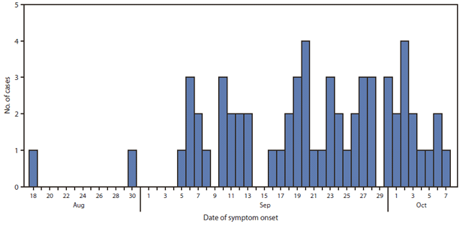
\includegraphics[width=3.5in]{fungal-outbreak.png}}

Based on the graph, answer these questions.

\begin{enumerate}[(a)]

\item What kind of graph is this?
\begin{MultipleChoice}
\wrong{Prevalence of the fungal infection.}
\wrong{Incubation graph of the fungal infection.}
\correct{Epidemic curve of the fungal infection.}
\end{MultipleChoice}

\item Estimate the incubation period.  If an estimate can't be made from the information provided, say what is missing.

\answerSpace{2cm}

\item What is the $R_0$ for this epidemic?  If an estimate can't be made or if $R_0$ is not applicable, say why.

\answerSpace{2cm}

\item Which of the following is the most likely time path for the epidemic, based on the data available?
\begin{MultipleChoice}
\wrong{The epidemic is coming to a close.}
\wrong{There will be another wave of cases near the end of October.}
\wrong{The epidemic will grow exponentially, doubling roughly every month.}
\correct{Without knowing the incubation time, no good prediction can be made.}
\end{MultipleChoice}

\end{enumerate}